\usetikzlibrary {positioning}
\definecolor{red}{HTML}{8A3F3A}
\definecolor{yellow}{HTML}{E0BB3C}
\definecolor{blue}{HTML}{4569E0}
\definecolor{green}{HTML}{17E561}
\definecolor{other}{HTML}{6A939E}

% DTU Colors
\definecolor{dtu-corporate-red}{HTML}{990000}
\definecolor{dtu-white}{HTML}{ffffff}
\definecolor{dtu-black}{HTML}{000000}
\definecolor{dtu-blue}{HTML}{2F3EEA}
\definecolor{dtu-bright-green}{HTML}{1FD082}
\definecolor{dtu-navy-blue}{HTML}{030F4F}
\definecolor{dtu-yellow}{HTML}{F6D04D}
\definecolor{dtu-orange}{HTML}{FC7634}
\definecolor{dtu-pink}{HTML}{F7BBB1}
\definecolor{dtu-grey}{HTML}{DADADA}
\definecolor{dtu-red}{HTML}{E83F48}
\definecolor{dtu-green}{HTML}{008835}
\definecolor{dtu-purple}{HTML}{79238E}


\newcommand{\drawHexagon}[4]{
	\draw[fill=#3] (#1,#2) ++(30:2) -- ++(90:2) -- ++(150:2) -- ++(210:2) -- ++(270:2) -- ++(330:2) -- cycle;
	\node at (#1,#2+2) {#4};
}

\newcommand{\drawModelSetupHexagon}{
	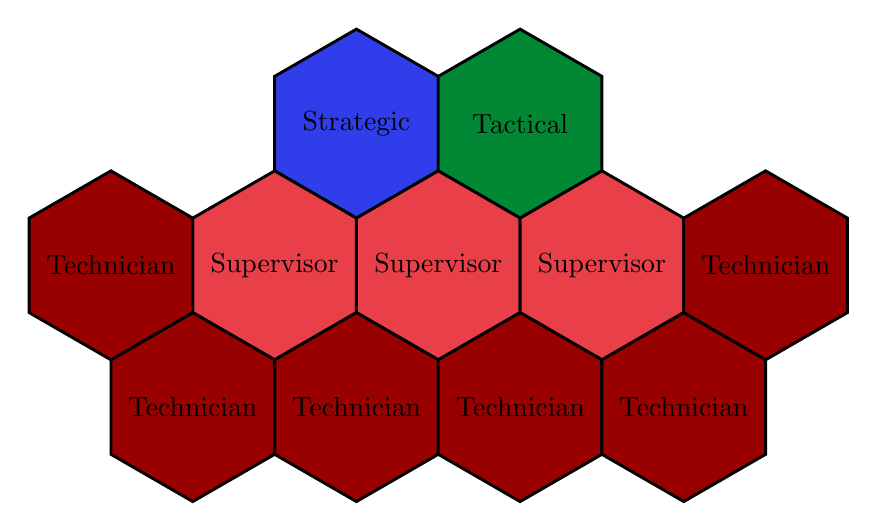
\begin{tikzpicture}[scale=0.6, line width=1.05][]

	% We should parameterize this! I think that is the best approach!
	\drawHexagon{ 2                      }{ 2}{dtu-blue}         {Strategic}
	\drawHexagon{{6 - 2 * (2 - sqrt(3)) }}{ 2}{dtu-green}        {Tactical}
	\drawHexagon{{4 - 1 * (2 - sqrt(3)) }}{-1}{dtu-red}          {Supervisor}
	\drawHexagon{{0 + 1 * (2 - sqrt(3)) }}{-1}{dtu-red}          {Supervisor}
	\drawHexagon{{8 - 3 * (2 - sqrt(3)) }}{-1}{dtu-red}          {Supervisor}

	\drawHexagon{{2 - 0 * (2 - sqrt(3)) }}{-4}{dtu-corporate-red}{Technician}
	\drawHexagon{{6 - 2 * (2 - sqrt(3)) }}{-4}{dtu-corporate-red}{Technician}

	\drawHexagon{{10 - 4 * (2 - sqrt(3)) }}{-4}{dtu-corporate-red}{Technician}
	\drawHexagon{{-2 + 2 * (2 - sqrt(3)) }}{-4}{dtu-corporate-red}{Technician}

	\drawHexagon{{12 - 5 * (2 - sqrt(3)) }}{-1}{dtu-corporate-red}{Technician}
	\drawHexagon{{-4 + 3 * (2 - sqrt(3)) }}{-1}{dtu-corporate-red}{Technician}

	

	% \node at (0.0 , 1) [above] {Static};
    % \draw (-3.0,  -2.0) -- ( 3.0,  -2.0);
	% \draw ( 0.0, -5.0) -- ( 0.0,  1.0);
	% \draw ( 0.0,  -2.0) circle [radius=2cm];
	% \draw[dashed] ( 0.0,  -2.0) circle [radius=3.0cm];
	% \node[blue] at (1.8, 0.5) [circle, fill, inner sep=2pt]{};
	% \draw[red] (0.0, -2.0) -- ++(45:2.0);

	% \node at (7.0 , 1) [above] {Dynamic};
    % \draw ( 4.0,  -2.0) -- (10.0, -2.0);
	% \draw ( 7.0, -5.0) -- ( 7.0, 1.0);
	% \draw ( 7.0,  -2.0) circle [radius=2cm];
	% \draw[dashed] ( 7.0,  -2.0) circle [radius=3.0cm];
	% \node[blue] at (8.8, 0.5) [circle, fill, inner sep=2pt]{};
	% \filldraw[fill=green!20,draw=green!50!black] (7,-2) -- ++(30:2.cm)
	%         arc [start angle=30, end angle=68, radius=2.cm] -- cycle;

	
	% \begin{scope}[shift={(10.5,0.5)}]
	% 	% \node at (-0.25,1) [right] {};
	% 	\draw[color=red,fill] (0,0.0)  rectangle  (0.5, -0.5);
	% 	\node[anchor=west] at (0.5, -0.25) { Static Solution };

	% 	\draw[color=green,fill] (0,-1.0)  rectangle  (0.5, -1.5);
	% 	\node[anchor=west] at (0.5, -1.25) { Dynamic Solution };

	% 	\draw[color=blue,fill] (0,-2.0)  rectangle  (0.5, -2.5);
	% 	\node[anchor=west] at (0.5, -2.25) { Unknown Optimal };

	% 	\draw[color=black] (0.25,-3.25)  circle  (0.25);
	% 	\node[anchor=west] at (0.5, -3.25) { Solution Space };

	% 	\draw[color=black,dashed] (0.25,-4.25)  circle  (0.25);
	% 	\node[anchor=west] at (0.5, -4.25) { Unknown Solution Space };

		
	% \end{scope}

    % \shade[ball color=red!50!white,opacity=0.8] (0,0) -- (90:\radius) arc (90:-90:\height) -- cycle;

	\end{tikzpicture}
}

